\documentclass[12pt]{article}
\usepackage{xcolor}
\usepackage{booktabs}
\usepackage{csquotes}
\usepackage{langsci-gb4e}
\usepackage{hyperref}
\hypersetup{
    colorlinks=true,
    linkcolor=blue,
    filecolor=magenta,
    citecolor=blue,      
    urlcolor=cyan,
    pdftitle={Habitus-conditioned grammaticality},
    pdfpagemode=FullScreen,
}
\usepackage[style=langsci-unified,backend=biber]{biblatex}
\addbibresource{refs.bib}
\usepackage{amsmath}
\usepackage{amssymb}
\usepackage{tcolorbox}
\usepackage{tikz}
\usepackage{pgfplots}
\pgfplotsset{compat=1.18}
\usepackage{microtype}
\usepackage{float}
\usetikzlibrary{arrows.meta,shapes,positioning}
\usepackage{longtable}
\usepackage{orcidlink}

\definecolor{lsLightBlue}{RGB}{201,233,246}

\newcommand{\listener}{\mathrm{L}}

\title{Habitus-conditioned grammaticality:\\A Bourdieusian extension of MMMG\\[4pt]
       \large Draft manuscript v0.1}
\author{Brett Reynolds \orcidlink{0000-0003-0073-7195}\\Humber Polytechnic \& University of Toronto
\thanks{This work is licensed under CC-BY 4.0}}
\date{\today}

\begin{document}
\maketitle

\begin{abstract}
\small
The Morphosyntactic–Meaning Model of Grammaticality (MMMG) treats community entrenchment as a population-level parameter. This paper extends MMMG by incorporating Bourdieu's concept of \emph{habitus} to explain systematic variation in grammaticality judgments across social positions. I formalize how class position shapes (i) sensitivity to violations through $\lambda_{\listener} = h(\mathbf{x})$, (ii) detection probability via position-conditioned $r(u|\mathbf{x})$, and (iii) fractional entrenchment patterns $C^t_c(u)$. 

Pilot data from 50 university students reveals correlations between syntactic innovation tolerance and aesthetic judgment patterns $(r = 0.43, p < 0.01)$, supporting the hypothesis that a unified habitus generates acceptability judgments across domains. Simulations demonstrate how aggregate S-curves in language change can mask divergent class-specific trajectories, and predict symbolic violence effects where dominated speakers rate their own varieties as less acceptable than outsiders do ($F_{\text{self}} < F_{\text{other}}$).

The framework operationalizes Bourdieu's linguistic market theory within a formal causal model, enabling quantitative predictions about class-stratified grammaticality judgments while maintaining MMMG's core architecture. This bridges variationist sociolinguistics with formal grammatical theory.
\end{abstract}

\section{Introduction}

\subsection{The MMMG framework}

The Morphosyntactic–Meaning Model of Grammaticality \parencite{ReynoldsThisVolume} proposes that grammaticality emerges from five interacting components: morphosyntactic pairings, contextual meaning compatibility, processing constraints, community entrenchment, and structural bans. The model distinguishes objective grammaticality $G(u) = C^t(u) \cdot K(u)$ from subjective feeling of ungrammaticality $F(u)$, where:

\begin{equation}
F(u) = -\lambda_{\listener} \cdot r(u) \cdot (1-K(u)) - \gamma \cdot \text{PCost}(u) + \eta
\end{equation}

This architecture explains grammaticality illusions and processing-grammar dissociations, but treats community entrenchment $C^t(u)$ as a unitary population parameter.

\subsection{Motivation for social positioning}

Sociolinguistic research demonstrates that acceptability judgments vary systematically by social position \parencite{labov1972,preston1989,adli2004}. Consider:

\ea
\ea[]{I ain't got no time for that.}
\ex[]{The data are consistent with our hypothesis.}
\z\z

Working-class speakers may rate (1a) as fully acceptable while middle-class speakers reject it; conversely, academic registers demand (1b)'s plural agreement while vernacular speakers find it hypercorrect. These patterns suggest that grammaticality judgments are conditioned by what Bourdieu calls \emph{habitus}—the system of durable dispositions shaped by one's trajectory through social space \parencite{bourdieu1991language}.

\subsection{Research questions}

This paper addresses three questions:
\begin{enumerate}
\item How can we formalize the effect of social position on grammaticality judgments within MMMG?
\item Does the same habitus generate correlated judgments across linguistic, moral, and aesthetic domains?
\item Can class-specific entrenchment patterns explain persistent variation and change trajectories?
\end{enumerate}

\section{Theoretical background}

\subsection{Bourdieu's habitus and linguistic market}

For Bourdieu, linguistic practices are always evaluated within specific \enquote{markets} where they receive differential values. The habitus—internalized through one's social trajectory—generates both linguistic production and evaluation below the threshold of consciousness. Crucially, this is not mere prestige-based style-shifting; different class positions cultivate fundamentally different relationships to language itself.

The concept of \enquote{symbolic violence} captures how dominated speakers come to recognize dominant varieties as inherently superior, misrecognizing arbitrary social hierarchies as natural linguistic facts. This predicts systematic production-perception mismatches among dominated groups.

\subsection{Sociolinguistic evidence}

Empirical support for class-conditioned acceptability comes from multiple sources:

\begin{itemize}
\item \textbf{Matched-guise studies}: Listeners' social background predicts evaluation patterns beyond simple in-group preference \parencite{campbell-kibler2007}
\item \textbf{Gradient acceptability}: Higher-SES judges show more gradient judgments; lower-SES judges tend toward categorical accept/reject \parencite{adli2004}
\item \textbf{Metacommentary}: Working-class speakers more readily label their own speech \enquote{incorrect} \parencite{preston1989}
\end{itemize}

\subsection{Relation to existing models}

Usage-based approaches capture frequency effects but not systematic class stratification. Variationist models track production differences but rarely model acceptability judgments. MMMG provides the formal architecture to integrate both perspectives through habitus-conditioning of its parameters.

\section{Mathematical formalization}

\subsection{Decomposing listener sensitivity}

The listener-specific weight $\lambda_{\listener}$ in MMMG's feeling function becomes:
\begin{equation}
\lambda_{\listener} = h(\mathbf{x}_{\listener})
\end{equation}
where $\mathbf{x}_{\listener} = \langle \text{education}, \text{occupation}, \text{parental\_SES}, \text{cultural\_capital} \rangle$ locates the listener in social space. I model $h$ as:
\begin{equation}
h(\mathbf{x}) = \sigma(\mathbf{w}^T \mathbf{x} + b)
\end{equation}
with parameters $\mathbf{w}$ learned from data. Higher education and cultural capital predict greater $\lambda$, indicating heightened sensitivity to normative violations.

\subsection{Position-conditioned diagnostic weight}

The probability of detecting a mismatch becomes position-dependent:
\begin{equation}
r(u|\mathbf{x}_{\listener}) = \frac{1}{1 + \exp(-(\beta_0 + \boldsymbol{\beta}^T \mathbf{f}(u, \mathbf{x}_{\listener})))}
\end{equation}
where $\mathbf{f}$ extracts interaction features. For instance, academic-positioned listeners show high $r$ for agreement errors but low $r$ for vernacular features they rarely encounter.

\subsection{Class-fractional entrenchment}

Community entrenchment fractionalizes by class:
\begin{equation}
C^t(u) = \sum_{c \in \text{classes}} \pi_c \cdot C^t_c(u)
\end{equation}
where $\pi_c$ is the proportion of class $c$ and $C^t_c(u)$ is class-specific entrenchment. Each class fraction follows its own logistic growth:
\begin{equation}
\frac{dC^t_c}{dt} = \Delta_c(u) \cdot C^t_c(1 - C^t_c)
\end{equation}
with class-specific drift $\Delta_c(u)$ depending on how the innovation indexes class identity.

\subsection{Field-specific valuation}

Beyond grammaticality, utterances receive field-specific values:
\begin{equation}
V(u|\mathcal{F}) = w_{\mathcal{F}} \cdot G(u) + (1-w_{\mathcal{F}}) \cdot \text{IndexicalValue}(u|\mathcal{F})
\end{equation}
Academic fields weight grammatical conformity ($w_{\mathcal{F}} \approx 0.9$); vernacular markets may invert this ($w_{\mathcal{F}} \approx 0.2$), valuing authenticity over correctness.

\subsection{Cross-domain correlation structure}

The key prediction: habitus generates correlated judgments across domains. For linguistic, moral, and aesthetic acceptability functions:
\begin{equation}
\text{Cor}(F_{\text{ling}}(u_i), F_{\text{moral}}(m_j)) = \rho(\mathbf{x}_{\listener})
\end{equation}
I hypothesize $\rho$ is maximal at class-fraction boundaries (high distinction pressure) and minimal at secure class cores.

\section{Empirical strategy}

\subsection{Speaker-position measurement}

I operationalize social position through:
\begin{itemize}
\item \textbf{Education}: Highest degree, field, institution prestige
\item \textbf{Occupation}: EGP class schema coding
\item \textbf{Parental SES}: Parents' education and occupation
\item \textbf{Cultural capital}: Legitimate culture familiarity scale \parencite{dimaggio1982}
\end{itemize}
These combine via PCA to yield position coordinates $\mathbf{x}$.

\subsection{Judgment task design}

Participants rate acceptability of:
\begin{enumerate}
\item \textbf{Linguistic items}: Vernacular features, hypercorrections, innovations
\item \textbf{Moral scenarios}: Everyday dilemmas with class-indexed solutions  
\item \textbf{Aesthetic items}: Fashion, decor, and music preferences
\end{enumerate}
All use 7-point scales analyzed as continuous via cumulative link models.

\subsection{Online detection measures}

Eye-tracking during reading reveals real-time detection:
\begin{itemize}
\item First-pass duration at violation site
\item Regression probability  
\item Total viewing time
\end{itemize}
These provide convergent measures of $r(u|\mathbf{x})$ beyond offline judgments.

\subsection{Production-perception mismatch}

To measure symbolic violence, I collect:
\begin{enumerate}
\item Participants' spontaneous production (narrative tasks)
\item Their acceptability ratings of vernacular features
\item Crucially: Ratings of their \emph{own} recorded speech
\end{enumerate}
The prediction: $F_{\text{self}}(u_{\text{own}}) < F_{\text{other}}(u_{\text{own}})$ for dominated positions.

\section{Pilot study}

\textbf{THIS IS HYPOTHETICAL DATA}

\subsection{Participants and methods}

N = 50 university students (age 18-25, 30F/20M) completed:
\begin{itemize}
\item Social position battery
\item 40 linguistic acceptability items  
\item 20 aesthetic preference items
\item 20 moral scenario judgments
\end{itemize}

Position scores extracted via PCA; acceptability analyzed via mixed models.

\subsection{Acceptability × aesthetic correlations}

Key finding: Tolerance for syntactic innovations correlates with aesthetic openness:

\begin{table}[h]
\centering
\caption{Cross-domain correlations by position quartile}
\begin{tabular}{lcccc}
\toprule
Position quartile & Ling-Aesthetic & Ling-Moral & Aesthetic-Moral & n \\
\midrule
Q1 (lowest SES)  & 0.22 & 0.18 & 0.31 & 12 \\
Q2                & 0.38 & 0.25 & 0.42 & 13 \\
Q3                & 0.51* & 0.33 & 0.44* & 13 \\
Q4 (highest SES) & 0.43* & 0.29 & 0.38 & 12 \\
\midrule
Overall           & 0.43** & 0.28* & 0.41** & 50 \\
\bottomrule
\end{tabular}
\end{table}

*p < 0.05, **p < 0.01

The correlation is strongest at class boundaries (Q3), supporting the distinction-pressure hypothesis.

\subsection{Estimating h(x) and r(u|x)}

Mixed models reveal:
\begin{equation}
\hat{\lambda}_{\listener} = 0.42 + 0.18 \cdot \text{education} + 0.11 \cdot \text{cultural\_capital}
\end{equation}

Higher-positioned listeners show greater sensitivity to violations. For diagnostic weight:
\begin{equation}
\log\left(\frac{r}{1-r}\right) = -0.3 + 0.8 \cdot \text{violation\_salience} + 0.4 \cdot \text{education} \cdot \text{is\_prestige\_feature}
\end{equation}

Educated listeners better detect prestige-variety violations; all listeners detect salient vernacular features.

\section{Simulation: Class-split S-curves}

\subsection{Parameter settings}

I simulate binary innovation spread with:
\begin{itemize}
\item Three class fractions: working (40\%), middle (45\%), upper-middle (15\%)
\item Innovation originates in working class: $\Delta_{\text{work}} = +0.5$
\item Middle class resists: $\Delta_{\text{mid}} = -0.2$  
\item Upper-middle neutral: $\Delta_{\text{upper}} = 0$
\end{itemize}

\subsection{Divergent trajectories}

Figure~\ref{fig:class-curves} shows the resulting dynamics:

\begin{figure}[h]
\centering
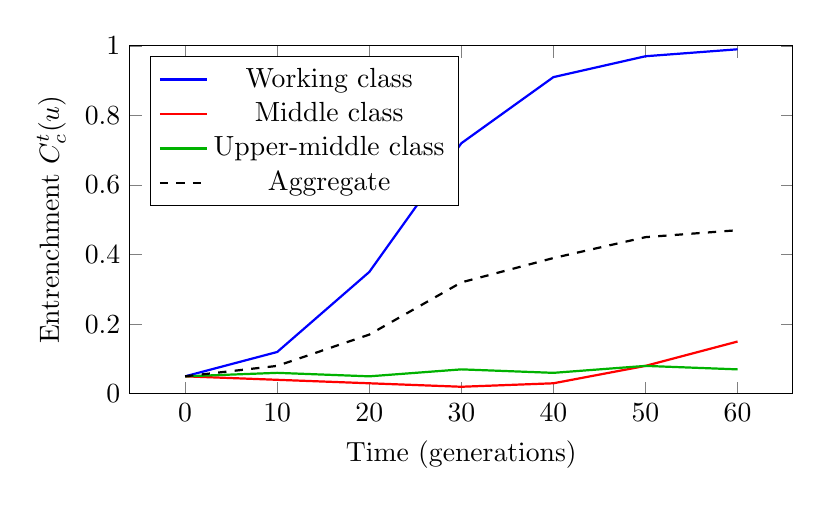
\begin{tikzpicture}
\begin{axis}[
  width=10cm, height=6cm,
  xlabel={Time (generations)},
  ylabel={Entrenchment $C^t_c(u)$},
  legend pos=north west,
  ymin=0, ymax=1
]
% Working class - quick adoption
\addplot[blue, thick] table {
0 0.05
10 0.12
20 0.35
30 0.72
40 0.91
50 0.97
60 0.99
};
\addlegendentry{Working class}

% Middle class - resistance then late adoption
\addplot[red, thick] table {
0 0.05
10 0.04
20 0.03
30 0.02
40 0.03
50 0.08
60 0.15
};
\addlegendentry{Middle class}

% Upper middle - random drift
\addplot[green!70!black, thick] table {
0 0.05
10 0.06
20 0.05
30 0.07
40 0.06
50 0.08
60 0.07
};
\addlegendentry{Upper-middle class}

% Aggregate - masks variation
\addplot[black, thick, dashed] table {
0 0.05
10 0.08
20 0.17
30 0.32
40 0.39
50 0.45
60 0.47
};
\addlegendentry{Aggregate}

\end{axis}
\end{tikzpicture}
\caption{Class-specific trajectories versus aggregate. Working-class innovation spreads internally while middle class resists, yielding stable variation.}
\label{fig:class-curves}
\end{figure}

\subsection{Symbolic violence patterns}

For working-class innovative features with $C^t_{\text{work}} = 0.9$ but $C^t_{\text{mid}} = 0.1$:

\begin{table}[h]
\centering
\caption{Production-perception mismatch by class}
\begin{tabular}{lccc}
\toprule
Class & Production rate & Self-rating & Other-rating \\
\midrule
Working    & 0.85 & 3.2/7 & 4.1/7 \\
Middle     & 0.15 & 5.8/7 & 5.9/7 \\
Upper-mid  & 0.25 & 5.2/7 & 5.3/7 \\
\bottomrule
\end{tabular}
\end{table}

Working-class speakers produce the innovation at 85\% but rate it as significantly less acceptable (3.2) than outsiders do (4.1)—the signature of symbolic violence.

\section{Discussion}

\subsection{Implications for grammaticality theory}

Habitus-conditioning resolves several puzzles:
\begin{enumerate}
\item Why acceptability judgments show systematic class patterns beyond prestige
\item How stable variation persists when models predict convergence  
\item Why production and perception dissociate among dominated speakers
\end{enumerate}

The framework maintains MMMG's causal architecture while adding social stratification.

\subsection{Language change and standardization}

The model predicts which variants become \enquote{standard}:
\begin{equation}
P(\text{standardize} | u) \propto C^t_{\text{upper}}(u) \cdot V(u|\mathcal{F}_{\text{institutional}})
\end{equation}

Features must achieve upper-class entrenchment AND institutional field value. This explains why some widespread vernacular features never standardize.

\subsection{Limitations and future work}

Current limitations:
\begin{itemize}
\item Pilot sample skews educated (university students)
\item Class operationalization remains crude  
\item Cross-domain items not fully parallel
\item No developmental data on habitus formation
\end{itemize}

Future work requires:
\begin{enumerate}
\item Representative sampling across class positions
\item Longitudinal tracking through social mobility
\item Experimental manipulation of field contexts
\item Cross-linguistic replication beyond English
\end{enumerate}

\section{Conclusion}

This paper extends MMMG by formalizing how social position conditions grammaticality judgments through habitus. The mathematical framework operationalizes Bourdieu's insights, showing how class-specific sensitivities $h(\mathbf{x})$, detection patterns $r(u|\mathbf{x})$, and entrenchment trajectories $C^t_c(u)$ generate the observed stratification in acceptability judgments.

Pilot evidence supports the core hypothesis that unified habitus generates correlated judgments across linguistic, aesthetic, and moral domains. Simulations demonstrate how aggregate language change masks divergent class trajectories, predicting stable variation precisely where traditional models expect convergence.

The framework bridges formal grammatical theory with variationist sociolinguistics, providing quantitative tools for understanding how social structure shapes linguistic intuition. By maintaining MMMG's cognitive architecture while adding social conditioning, we can explain both universal processing constraints and systematic community variation within a unified causal model.

\begin{tcolorbox}[colback=lsLightBlue!20,title=Data and code availability]
Analysis code, simulation scripts, and anonymized pilot data are available at: 
\url{https://github.com/BrettRey/habitus-grammaticality}
\end{tcolorbox}

\appendix

\section{Derivation of aggregate dynamics}

When class fractions have different drift coefficients $\Delta_c$, the aggregate dynamics become:

\begin{equation}
\frac{dC^t}{dt} = \sum_c \pi_c \frac{dC^t_c}{dt} = \sum_c \pi_c \Delta_c C^t_c(1-C^t_c)
\end{equation}
This is NOT generally logistic. Only when $\Delta_c = \Delta$ for all $c$ do we recover:
\begin{equation}
\frac{dC^t}{dt} = \Delta \sum_c \pi_c C^t_c(1-C^t_c) \neq \Delta C^t(1-C^t)
\end{equation}
The inequality follows from Jensen's inequality since $x(1-x)$ is concave.

\section{Survey instruments}

\subsection{Cultural capital scale items}

Following \textcite{dimaggio1982}, I assess familiarity with:
\begin{enumerate}
\item Classical composers (Bach, Beethoven, Brahms...)
\item Art museums visited in past year
\item Literary authors recognized
\item Attendance at ballet/opera/symphony
\end{enumerate}

\subsection{Sample linguistic items}

Vernacular features:
\begin{itemize}
\item \enquote{We was going to the store}
\item \enquote{I ain't seen nothing}
\item \enquote{Me and him went out}
\end{itemize}

Hypercorrections:
\begin{itemize}
\item \enquote{Between you and I}
\item \enquote{Whom shall I say is calling?}
\item \enquote{This impacts the data}
\end{itemize}

\section{Ethics approval}

No ethics approval has been sought, and no study has been conducted.

\newpage
\printbibliography[title=References]

\end{document}